\chapter{Dimensionamento delle membrature}
Il dimensionamento delle membrature, o calcolo elettrico di una linea o di una rete di distribuzione, consiste nel \textbf{determinare le sezioni dei conduttori} in modo che risultino soddisfatte specifiche condizioni di esercizio e di sicurezza (calcolo preliminare) oppure nel verificare la rispondenza a tali condizioni una volta assegnate a priori le sezioni dei conduttori (calcolo di verifica). Tra i vincoli assunti per il calcolo preliminare rientra la vita utile del cavo; il calcolo di verifica viene invece tipicamente eseguito a fronte di un potenziale ampliamento o potenziamento dell'impianto esistente.

Le correnti utilizzate per i calcoli, denominate \textbf{correnti di impiego}, corrispondono alle condizioni di massimo carico previsto, opportunamente corrette mediante fattori di utilizzazione e di contemporaneità nel caso di linee che alimentano una pluralità di utilizzatori.

\section{Calcolo delle correnti di impiego}
La corrente di impiego, indicata con $I_B$, rappresenta l'intensità di corrente che può fluire in un circuito in condizioni di servizio ordinario. Essa dipende dal numero degli utilizzatori, dalla potenza installata, dal livello di tensione, dal fattore di potenza e dal rendimento. Può essere definita come la corrente che deve circolare all'interno del conduttore per un tempo indefinito, intendendo con tale espressione l'orizzonte temporale assunto come vita utile di progetto del conduttore stesso.

\subsection{Definizione e calcolo in regime permanente}
In regime permanente, la corrente di impiego coincide con la massima corrente trasportata dal circuito in servizio ordinario. Per un carico trifase generico, l'espressione analitica è:
\[ I_B = \frac{P}{\sqrt{3} V \cos\varphi \cdot \eta} k_u \]
dove:
\begin{itemize}
    \item \textbf{$P$} $\rightarrow$ potenza attiva assorbita dai carichi alimentati dalla linea [W o kW].
    \item \textbf{$V$} $\rightarrow$ tensione nominale concatenata del sistema [V].
    \item \textbf{$\cos\varphi$} $\rightarrow$ fattore di potenza del carico.
    \item \textbf{$\eta$} $\rightarrow$ rendimento complessivo degli utilizzatori, pari al rapporto tra la potenza resa ($P_{\text{out}}$) e la potenza assorbita ($P_{\text{in}}$).
    \item \textbf{$k_u$} $\rightarrow$ fattore di utilizzazione, definito come il rapporto tra la potenza effettivamente assorbita e la potenza nominale di targa ($0 < k_u \le 1$), introdotto per prevenire il sovradimensionamento dei conduttori.
\end{itemize}

\subsection{Regime variabile e corrente termicamente equivalente}
Nei casi in cui la potenza attiva richiesta vari nel tempo (ad esempio per effetto delle fluttuazioni di carico nell'arco della giornata), il dimensionamento non può fare riferimento a un valore costante statico. Si ricorre pertanto al concetto di \textbf{corrente termicamente equivalente}, calcolata come valore quadratico medio, ossia quel valore costante di corrente che, circolando in regime permanente continuo per la medesima durata, produrrebbe negli elementi del circuito le medesime perdite per effetto Joule e quindi lo stesso riscaldamento.

Per correnti periodiche ad andamento continuo nel tempo con periodo $T$, la corrente di impiego equivalente si esprime come:
\[ I_b = \sqrt{\frac{1}{T} \int_{t}^{t+T} i^2(t) \, dt} \]

Nel caso pratico in cui il profilo di carico reale sia discretizzato e scomponibile in $N$ intervalli temporali discreti $t_i$ entro i quali l'intensità di corrente si mantiene costante a un valore $I_i$, la relazione si traduce in:
\[ I_b = \sqrt{\frac{1}{T} \sum_{i=1}^{N} I_i^2 \cdot t_i} \]

\subsection{Fattore di contemporaneità per linee con più carichi}
Qualora una linea alimenti una pluralità di carichi distinti, la corrente di impiego complessiva della linea è determinata moltiplicando la somma delle correnti di impiego dei singoli carichi per il fattore di contemporaneità $k_c$:
\begin{itemize}
    \item \textbf{Fattore di contemporaneità ($k_c$)} $\rightarrow$ definito come il rapporto tra la massima potenza assorbita contemporaneamente dall'insieme dei carichi e la somma delle potenze nominali installate.
\end{itemize}

\subsection{Metodo pratico per il calcolo della corrente massima di impiego}
Nella pratica progettuale degli impianti, il calcolo della corrente massima di impiego $I_B$ di un circuito viene effettuato secondo la formulazione empirica normalizzata:
\[ I_B = P \cdot a \cdot b \cdot c \cdot d \cdot e \]
dove $P$ rappresenta la potenza dell'apparecchio utilizzatore espressa in kW, mentre i coefficienti correttivi assumono i seguenti significati e valori:
\begin{itemize}
    \item \textbf{Fattore $a$ (legato al fattore di potenza)} $\rightarrow$ tiene conto dello sfasamento introdotto dal tipo di utilizzatore ed è proporzionale a $1/\cos\varphi$. Un valore basso di $\cos\varphi$ denota la predominanza di potenza reattiva rispetto alla potenza attiva; per erogare la medesima potenza attiva è pertanto necessario incrementare la corrente di impiego $I_B$, rendendo il fattore $a$ inversamente proporzionale al fattore di potenza.
    \item \textbf{Fattore di utilizzazione $b$} $\rightarrow$ rapporto tra la potenza effettivamente impiegata e quella nominale.
    \item \textbf{Fattore di contemporaneità $c$} $\rightarrow$ quota di utilizzatori contemporaneamente in funzione.
    \item \textbf{Fattore per ampliamenti futuri $d$} $\rightarrow$ margine di sovradimensionamento legato alle previsioni di estensione dell'impianto ($d = 1$ in generale; $d = 1{,}2$ per installazioni industriali).
    \item \textbf{Fattore di conversione $e$} $\rightarrow$ parametro per convertire la potenza attiva (espressa in kW) nella corrispondente intensità di corrente (espressa in A):
    \begin{itemize}
        \item Per reti monofase a 230 V: $e = \frac{1000}{230} \approx 4{,}35$.
        \item Per reti trifase a 400 V: $e = \frac{1000}{\sqrt{3} \cdot 400} \approx 1{,}4$.
    \end{itemize}
\end{itemize}

I valori specifici dei fattori $a, b, c$ sono determinati in base alla natura dei carichi:
\begin{itemize}
    \item \textbf{Fattore $a$ per apparecchi di illuminazione rifasati ($\cos\varphi \ge 0{,}9$ a 230 V)}:
    \begin{figure}[H]
    	\centering
    	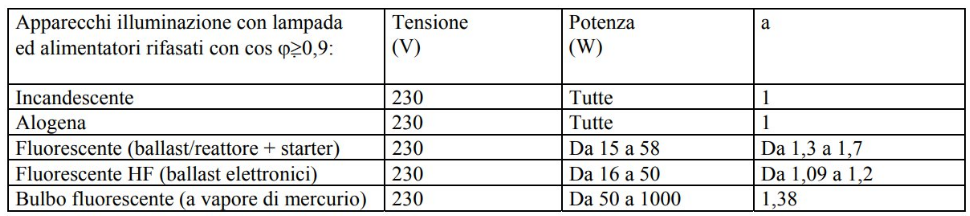
\includegraphics[width=0.8\linewidth]{immagini/dimensionamento_membrature}
    \end{figure}
   
    \item \textbf{Fattore $a$ per utilizzatori a motore}: presentano comportamento ohmico-induttivo con $\cos\varphi < 1$, per cui $a > 1$, con un incremento al diminuire della taglia per il progressivo degrado del $\cos\varphi$:
   	\begin{figure}[H]
   		\centering
   		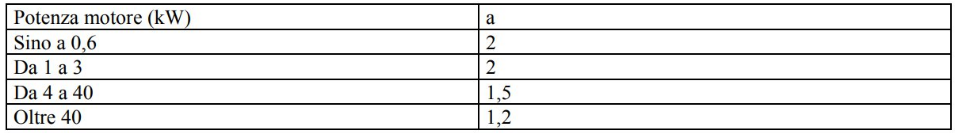
\includegraphics[width=0.8\linewidth]{immagini/dimensionamento_membrature1}
   	\end{figure}
   
    \item \textbf{Fattore di utilizzazione $b$}:
    \begin{figure}[H]
    	\centering
    	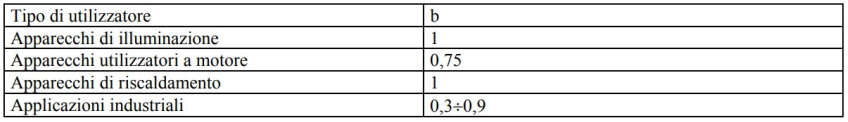
\includegraphics[width=0.8\linewidth]{immagini/dimensionamento_membrature2}
    \end{figure}
    
    \item \textbf{Fattore di contemporaneità $c$}:
    \begin{figure}[H]
    	\centering
    	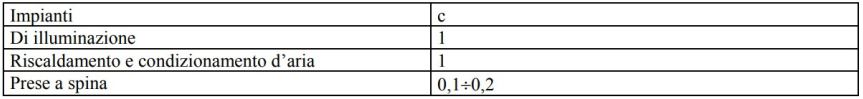
\includegraphics[width=0.8\linewidth]{immagini/dimensionamento_membrature3}
    \end{figure}
\end{itemize}

\subsection{Funzionamento e rifasamento delle lampade a scarica}
All'interno del bulbo delle lampade a scarica (ad esempio a vapore di mercurio) la generazione del fascio luminoso avviene tramite l'innesco di un arco elettrico. La superficie del bulbo è rivestita internamente da una patina fluorescente deputata a convertire la radiazione emessa nello spettro visibile, prevenendo pericoli di accecamento per gli utenti.
\begin{figure}[H]
	\centering
	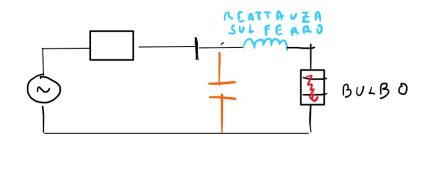
\includegraphics[width=0.5\linewidth]{immagini/dimensionamento_membrature4}
\end{figure}

L'accensione e il funzionamento stazionario del dispositivo richiedono opportuni accorgimenti circuitali:
\begin{enumerate}
    \item All'atto della chiusura dell'interruttore di alimentazione, si applica ai capi del dispositivo una differenza di potenziale impulsiva, enfatizzata dalla presenza del condensatore di rifasamento.
    \item L'innesco dell'arco provoca una caduta drastica dell'impedenza interna del bulbo, che si comporta elettricamente come un cortocircuito potenziale, suscettibile di danneggiare la rete.
    \item Per stabilizzare la scarica e limitare la corrente si inserisce in serie al bulbo una reattanza su nucleo di ferro (ballast induttivo). La reattanza assorbe la caduta di tensione provocata dalla dinamica d'arco, riducendo la tensione applicata ai morsetti del bulbo a un valore compatibile. L'impiego di una reattanza in luogo di un resistore dissipa una quantità minima di energia attiva, preservando il rendimento energetico globale.
    \item L'inserzione dell'induttanza serie causa tuttavia un rilevante assorbimento di potenza reattiva induttiva con sensibile abbattimento del fattore di potenza. Per compensare tale effetto si inserisce in parallelo alla rete un condensatore di rifasamento.
\end{enumerate}

\section{Criteri generali di dimensionamento}
La determinazione della sezione dei conduttori di una linea o rete di distribuzione si articola su tre criteri fondamentali:
\begin{itemize}
    \item \textbf{Criterio elettrico (o della massima caduta di tensione)} $\rightarrow$ impone che la caduta di tensione percentuale tra partenza e arrivo non ecceda limiti prestabiliti sia a vuoto che a pieno carico.
    \item \textbf{Criterio termico (o della massima sovratemperatura)} $\rightarrow$ impone che la densità di corrente non superi i valori limite compatibili con la tenuta termica del conduttore e dell'isolante a regime permanente e in sovraccarico.
    \item \textbf{Criterio economico (o del massimo tornaconto)} $\rightarrow$ individua la sezione che minimizza il costo complessivo di installazione sommato al costo capitalizzato delle perdite per effetto Joule lungo la vita utile dell'opera.
\end{itemize}

L'ambito di cogenza e l'interazione tra i criteri presentano specificità circuitali e impiantistiche ben definite:
\begin{itemize}
    \item Nelle reti di distribuzione in bassa tensione (BT), l'assenza di dispositivi di regolazione della tensione intermedi tra le sbarre di cabina secondaria e i carichi terminali (estremamente sensibili alle fluttuazioni) rende il criterio elettrico inderogabile e vincolante.
    \item Nelle reti di media tensione (MT), l'esistenza di sistemi e organi di regolazione della tensione rende spesso non vincolante il criterio elettrico in prima istanza, consentendo di dimensionare la linea secondo il criterio economico.
    \item Sebbene di norma il rispetto del criterio elettrico garantisca intrinsecamente la verifica termica, il criterio termico diventa l'unico vincolo dimensionante per tratte aeree corte di collegamento, per le linee in cavo (ove la dissipazione termica limitata degrada gravemente l'isolante) e per le sbarre di connessione di stazione o quadro.
    \item Nella pratica ingegneristica si ricorre usualmente a un procedimento ibrido: dimensionamento di prima approssimazione condotto con il criterio termico, seguito dalla verifica della caduta di tensione mediante il criterio elettrico.
\end{itemize}

\section{Criterio elettrico}
Il criterio elettrico impone che la massima caduta di tensione $\Delta V$ lungo l'intera estensione dell'impianto di distribuzione si mantenga al di sotto di un valore massimo prefissato, denominato caduta di tensione ammissibile $\Delta V_{\text{amm}}$:
\[ \Delta V \le \Delta V_{\text{amm}} \]

Nel modello equivalente di linea corta (rappresentata da un'impedenza serie ohmico-induttiva $R + jX$ trascurando le ammettenze trasversali), la caduta di potenziale dipende essenzialmente dalla resistenza longitudinale $R = \rho L / S$, la quale è inversamente proporzionale alla sezione $S$. Il contenimento della caduta entro valori di tolleranza assicura la salvaguardia e la piena funzionalità dei carichi:
\begin{itemize}
    \item Le lampade e gli apparati illuminanti risultano degradati nella vita utile da aumenti di tensione, mentre subiscono una repentina riduzione del flusso luminoso emesso a fronte di abbassamenti di tensione.
    \item I motori asincroni subiscono una variazione della coppia motrice proporzionale al quadrato della tensione di alimentazione; a parità di coppia resistente richiesta dal carico meccanico, una riduzione di tensione comporta un incremento dello scorrimento, con conseguente aumento della corrente assorbita e delle perdite per effetto Joule nel rotore e nello statore.
\end{itemize}

I limiti massimi normativi della caduta di tensione ammissibile, espressi in percentuale rispetto alla tensione nominale di rete, sono pari a:
\begin{itemize}
    \item Per reti in bassa tensione (BT): $\Delta V_{\text{amm}} \le 4 \div 6\%$.
    \item Per reti in media tensione (MT): $\Delta V_{\text{amm}} \le 5 \div 7\%$.
\end{itemize}

\subsection{Caduta di tensione industriale}
La caduta di tensione industriale non corrisponde al modulo del fasore della differenza vettoriale $|\Delta\bar{V}| = |(R + jX)\bar{I}|$, bensì alla differenza algebrica scalare tra il modulo della tensione stellata (o concatenata) di partenza e il modulo della tensione di arrivo ai morsetti del carico:
\[ \Delta V = V_i - V \]

\begin{figure}[H]
	\centering
	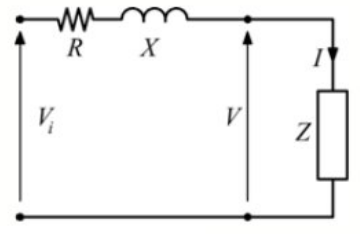
\includegraphics[width=0.35\linewidth]{immagini/dimensionamento_membrature5}
\end{figure}

Fissando il fasore della tensione di arrivo $\bar{V}$ come riferimento di fase sull'asse reale, la tensione di partenza si esprime vettorialmente come:
\[ \bar{V}_i = \bar{V} + (R + jX)\bar{I} \]
Per un carico di tipo ohmico-induttivo, il fasore di corrente $\bar{I}$ si trova in ritardo di fase dell'angolo $\varphi$ rispetto a $\bar{V}$. Proiettando le singole componenti della caduta di tensione lungo la direzione del fasore $\bar{V}$:
\begin{itemize}
    \item Segmento $AB = R I \cos\varphi$ $\rightarrow$ proiezione della caduta di tensione puramente resistiva.
    \item Segmento $BC = X I \sin\varphi$ $\rightarrow$ proiezione della caduta di tensione puramente reattiva.
    \item Segmento $AD = AB + BC + CD$ $\rightarrow$ lunghezza totale corrispondente alla differenza algebrica $V_i - V$, ricavata tracciando un arco di circonferenza di raggio $V_i$ centrato nell'origine $O$ fino all'intersezione con l'asse di riferimento.
\end{itemize}
\begin{figure}[H]
	\centering
	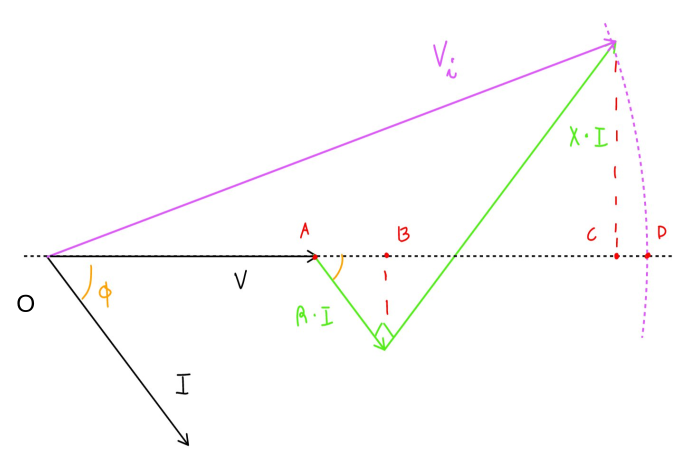
\includegraphics[width=0.6\linewidth]{immagini/dimensionamento_membrature6}
\end{figure}
Nelle applicazioni impiantistiche reali, l'angolo di sfasamento vettoriale tra la tensione di partenza $\bar{V}_i$ e la tensione di arrivo $\bar{V}$ assume valori trascurabili; di conseguenza, la lunghezza del segmento differenziale $CD$ risulta infinitesima rispetto agli altri termini e può essere omessa. L'espressione della caduta di tensione industriale approssimata si riduce a:
\[ \Delta V \approx R I \cos\varphi + X I \sin\varphi \]

Moltiplicando ambo i membri per il modulo della tensione $V$, si evidenzia il legame con la potenza attiva $P = V I \cos\varphi$ e reattiva $Q = V I \sin\varphi$:
\[ V \cdot \Delta V = P \cdot R + Q \cdot X \]

La relazione mostra che l'aliquota di corrente $I \sin\varphi$, associata allo scambio di potenza reattiva induttiva tra generatore e carico, incrementa la caduta di tensione e sovraccarica la rete senza concorrere all'erogazione di lavoro utile. Il rifasamento locale del carico, attuato tramite batterie di condensatori in parallelo, annulla o riduce il termine $Q \cdot X$, contenendo la caduta di potenziale.

Le perdite di potenza attiva lungo la linea e il conseguente rendimento si esprimono mediante le relazioni:
\begin{itemize}
    \item Perdita di potenza attiva assoluta e percentuale:
    \[ \Delta P = P_i - P, \qquad P\% = \frac{\Delta P}{P} \cdot 100 \]
    \item Rendimento complessivo di trasmissione della linea:
    \[ \eta = \frac{P}{P_i} = 1 - \frac{\Delta P}{P_i} \]
\end{itemize}

\subsection{Linee e reti con fattore di potenza unitario}
Nei casi ideali in cui i carichi operino con fattore di potenza unitario ($\cos\varphi = 1$, corrispondente a un carico puramente resistivo o a un circuito in corrente continua), la componente reattiva si annulla identicamente ($Q = 0$), e la caduta industriale dipende unicamente dai parametri di resistenza longitudinale:
\[ \Delta V = R \cdot I \]

\subsubsection{Linea con carico concentrato di estremità}
Considerando una linea di lunghezza totale $L$ che alimenta un singolo carico terminale assorbente la corrente di impiego $I$:
\begin{figure}[H]
	\centering
	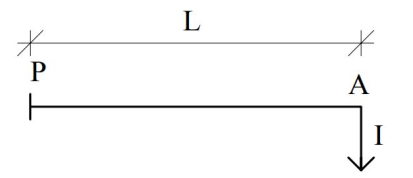
\includegraphics[width=0.3\linewidth]{immagini/dimensionamento_membrature7}
\end{figure}

La massima caduta di tensione vale:
\[ \Delta V = R \cdot I = K \rho \frac{L}{S} I \]
dove $\rho$ indica la resistività del conduttore e $K$ rappresenta un coefficiente geometrico-funzionale definito da:
\[ K = \begin{cases} 2 & \text{per linea monofase} \\ 1 & \text{per linea trifase} \end{cases} \]
\begin{itemize}
    \item Nella linea trifase simmetrica ed equilibrata, ciascuna sezione concorre al trasferimento della potenza della propria fase e le cadute si valutano sulla singola fase stellata senza corrente di ritorno nel conduttore neutro ($K = 1$).
    \item Nella linea monofase, l'intera corrente percorre sia il conduttore attivo di andata sia il conduttore di ritorno, raddoppiando l'impedenza ohmica complessiva di anello ($K = 2$).
\end{itemize}

Definendo il momento elettrico $M_P$ della corrente rispetto al nodo di alimentazione $P$ come:
\[ M_P = L \cdot I \]
la caduta di tensione assume la forma:
\[ \Delta V = K \rho \frac{M_P}{S} \]

Imponendo il vincolo sulla caduta ammissibile $\Delta V \le \Delta V_{\text{amm}}$, la sezione minima del conduttore risulta:
\[ S \ge \frac{K \rho M_P}{\Delta V_{\text{amm}}} \]
Il valore calcolato non coincide in generale con un valore standard unificato; la sezione definitiva viene scelta adottando la sezione nominale commerciale immediatamente superiore (approssimazione per eccesso).

\subsubsection{Linea con carichi concentrati lungo il percorso}
Nel caso di una dorsale lungo la quale siano distribuiti $n$ carichi concentrati assorbenti correnti $I_i$, posti a distanze progressive rispetto all'origine di alimentazione $P$:
\begin{figure}[H]
	\centering
	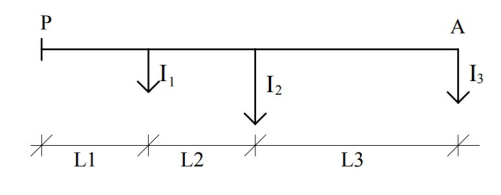
\includegraphics[width=0.4\linewidth]{immagini/dimensionamento_membrature8}
\end{figure}

Sebbene dal punto di vista meramente teorico una linea a sezione decrescente a gradini possa apparire economicamente vantaggiosa, nella pratica esecutiva si adotta una sezione costante uniforme per l'intera tratta:
\[ S_1 = S_2 = \dots = S_n = S \]

Applicando il principio di sovrapposizione degli effetti, la linea reale viene scomposta nella somma di $n$ linee indipendenti aventi ciascuna un carico all'estremità.
\begin{figure}[H]
	\centering
	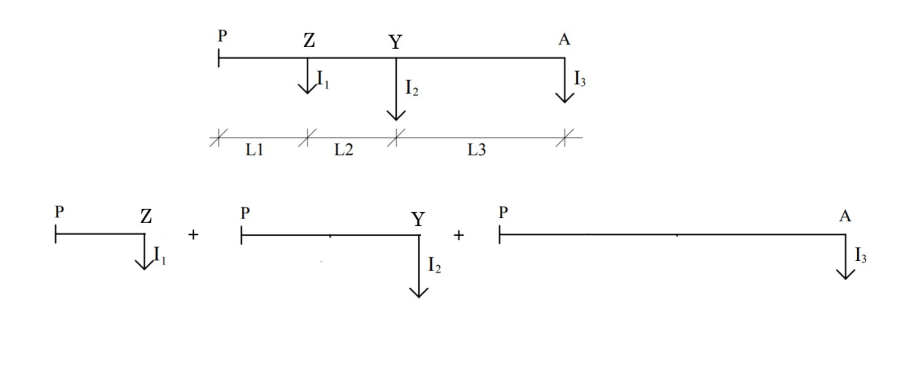
\includegraphics[width=0.8\linewidth]{immagini/dimensionamento_membrature10}
\end{figure}
La caduta di tensione totale nel nodo terminale più lontano $A$ è determinata dalla sommatoria dei singoli momenti elettrici calcolati rispetto al nodo $P$:
\[ \Delta V = K \frac{\rho}{S} \sum_{i=1}^{n} M_{Pi} \]
dove $M_{Pi} = L_i I_i$ rappresenta il momento elettrico dell'utilizzatore $i$-esimo.

Definendo una lunghezza baricentrica equivalente $L^*$ tale per cui:
\[ \sum_{i=1}^{n} M_{Pi} = L^* \sum_{i=1}^{n} I_i \]
\begin{figure}[H]
	\centering
	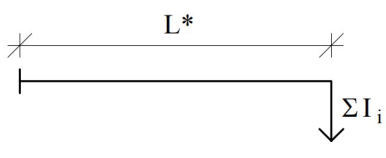
\includegraphics[width=0.3\linewidth]{immagini/dimensionamento_membrature9}
\end{figure}
l'espressione della caduta di tensione diventa:
\[ \Delta V = K \frac{\rho}{S} L^* \sum_{i=1}^{n} I_i \]
Ai fini del dimensionamento della sezione $S$, la linea con carichi distribuiti concentrati risulta formalmente equivalente a una linea di lunghezza fittizia $L^*$ caricata alla sua estremità con la somma di tutte le correnti di impiego.

\newpage
\subsubsection{Linea con carico uniformemente distribuito}
Nel caso in cui il carico sia distribuito con continuità lungo la tratta di lunghezza $L$, con una densità di corrente costante per unità di lunghezza indicata con $i$ [A/m]:
\begin{figure}[H]
	\centering
	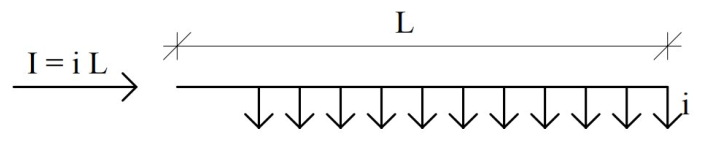
\includegraphics[width=0.6\linewidth]{immagini/dimensionamento_membrature11}
\end{figure}

La corrente totale erogata dalla linea è pari a $I = i \cdot L$. Ipotizzando una sezione uniforme lungo l'intera estensione, il dimensionamento si effettua individuando la distanza equivalente $L^*$ a cui concentrare idealmente l'intera corrente risultante:
\[ L^* = \frac{\int_{0}^{L} i_x \, dx}{i \cdot L} = \frac{\int_{0}^{L} i \cdot x \, dx}{i \cdot L} = \frac{\left[ i \frac{x^2}{2} \right]_{0}^{L}}{i L} = \frac{i L^2}{2 i L} = \frac{L}{2} \]
La linea a carico continuo uniforme si dimensiona pertanto come una linea con carico di estremità concentrato a metà campata ($L/2$) e percorso dalla corrente totale $I$.

\subsubsection{Reti radiali semplici}
In una rete ad albero con configurazione radiale pura alimentata direttamente dal nodo centrale di consegna $P$:
\begin{figure}[H]
	\centering
	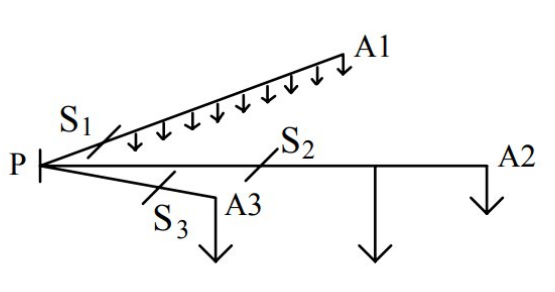
\includegraphics[width=0.4\linewidth]{immagini/dimensionamento_membrature12}
\end{figure}

Ciascun ramo della maglia viene ricondotto allo schema di linea elementare con carico di estremità. Per una rete costituita da $n$ rami si scrivono $n$ equazioni mutualmente indipendenti:
\[ \Delta V_i = K \frac{\rho}{S_i} M_{Pi} \qquad (i = 1, \dots, n) \]
Ciascun ramo radiale viene dimensionato in modo completamente autonomo rispetto agli altri rami imponendo $\Delta V_i \le \Delta V_{\text{amm}}$.

\subsubsection{Reti radiali con tratto di alimentazione comune}
Nel caso in cui la rete sia alimentata tramite una dorsale principale comune che si sviluppa dal punto di consegna $P$ fino a un nodo di smistamento intermedio $O$, da cui si dipartono $n$ rami radiali secondari verso i rispettivi terminali $A_i$:
\begin{figure}[H]
	\centering
	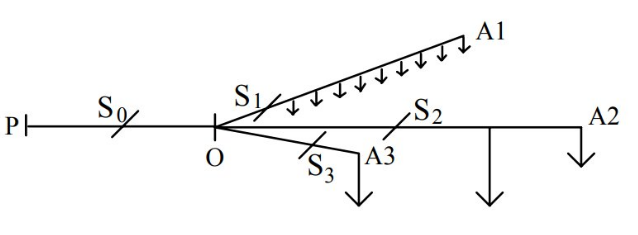
\includegraphics[width=0.6\linewidth]{immagini/dimensionamento_membrature13}
\end{figure}
La caduta di tensione massima totale tra la sorgente $P$ e il generico terminale d'utenza $A_i$ è pari alla somma della caduta sul tronco comune e della caduta sul ramo derivato:
\[ \Delta V = \Delta V_0 + \Delta V_i \]
Il sistema presenta $n + 1$ sezioni incognite ($S_0, S_1, \dots, S_n$) a fronte di sole $n$ equazioni di vincolo relative alle cadute di tensione dei singoli rami. Per rendere determinato il problema si adotta l'equazione ausiliaria di compatibilità economica:
\[ S_0 = \sum_{i=1}^{n} S_i \]

La caduta sul singolo ramo secondario vale:
\[ \Delta V_i = \Delta V - \Delta V_0 = K \frac{\rho}{S_i} M_{Oi} \]
dove $M_{Oi}$ rappresenta il momento elettrico delle correnti del ramo $i$-esimo calcolato assumendo come origine il nodo di derivazione $O$.

Poiché la caduta totale ammissibile $\Delta V$ e la caduta lungo il tronco comune $\Delta V_0$ sono univoche per tutti i terminali, la caduta parziale sui singoli rami deve assumere lo stesso valore:
\[ \Delta V_{i+1} = K \rho \frac{M_{O(i+1)}}{S_{i+1}} = \Delta V - \Delta V_0 = \Delta V_i \]
Ne consegue l'uguaglianza dei rapporti momento-sezione per tutti i rami:
\[ \frac{M_{Oi}}{S_i} = \frac{M_{O(i+1)}}{S_{i+1}} = \frac{1}{C} \implies S_i = C \cdot M_{Oi} \]
Sommando le sezioni di tutti i rami secondari:
\[ \sum_{i=1}^{n} S_i = \sum_{i=1}^{n} C M_{Oi} \implies S_0 = C \sum_{i=1}^{n} M_{Oi} \implies C = \frac{S_0}{\sum_{i=1}^{n} M_{Oi}} \]
da cui si esprime ciascuna sezione secondaria $S_i$ in funzione della sezione comune $S_0$:
\[ S_i = S_0 \frac{M_{Oi}}{\sum_{i=1}^{n} M_{Oi}} \]

Per il tronco dorsale comune $P-O$, percorso dall'intera corrente assorbita dalla rete, la caduta vale:
\[ \Delta V_0 = K \frac{\rho}{S_0} L_0 \sum_{i=1}^{n} I_i = K \frac{\rho}{S_0} M_P \]
Sostituendo l'espressione di $S_i$ nella relazione della caduta totale:
\[ \Delta V = \Delta V_0 + \Delta V_i = K \left[ \frac{\rho}{S_0} M_P + \frac{\rho}{S_i} M_{Oi} \right] \]
Poiché $\frac{M_{Oi}}{S_i} = \frac{\sum_{i=1}^{n} M_{Oi}}{S_0}$, si perviene a un'equazione in cui l'unica incognita è la sezione del tronco comune $S_0$:
\[ \Delta V = K \rho \left[ \frac{1}{S_0} M_P + \frac{\sum_{i=1}^{n} M_{Oi}}{S_0} \right] = \frac{K \rho}{S_0} \left[ M_P + \sum_{i=1}^{n} M_{Oi} \right] \]
Risolta l'equazione rispetto a $S_0$, le sezioni $S_i$ dei singoli rami si calcolano immediatamente mediante la relazione di ripartizione proporzionale precedentemente ricavata.

\subsection{Linee e reti con fattore di potenza non unitario}
Nel caso generale di carichi con fattore di potenza inferiore all'unità ($\cos\varphi < 1$), la caduta di tensione industriale è data da:
\[ \Delta V = R I \cos\varphi + X I \sin\varphi \]

La reattanza chilometrica $X$ di un conduttore dipende debolmente dalla sezione $S$, a differenza della resistenza ohmica $R$ che varia con legge iperbolica $1/S$. Tale andamento quasi costante è dovuto al fatto che l'induttanza specifica dipende dal logaritmo del rapporto tra l'interasse dei conduttori e il raggio del cavo ($\ln(D/r)$), funzione che comprime fortemente le variazioni geometriche. Inoltre, le linee aeree presentano una reattanza specifica $X_L$ nettamente superiore alla reattanza $X_C$ delle linee in cavo, a causa delle maggiori distanze di isolamento in aria rispetto alla stretta vicinanza delle anime nei cavi isolati.
\begin{figure}[H]
	\centering
	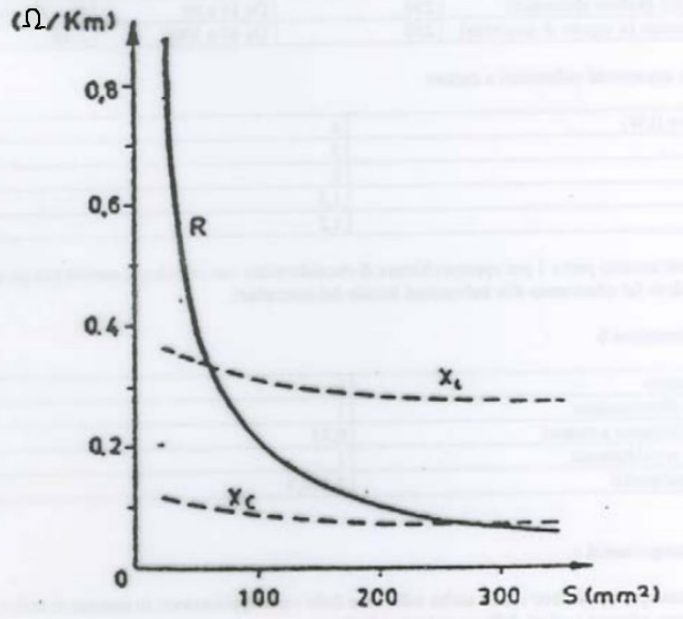
\includegraphics[width=0.4\linewidth]{immagini/dimensionamento_membrature14}
\end{figure}
Essendo noti a priori la corrente di impiego $I$, il fattore di sfasamento $\sin\varphi$ e l'ordine di grandezza della reattanza, il termine reattivo può essere trattato in prima approssimazione come una quantità costante:
\[ \text{cost} = X I \sin\varphi \]
Sostituendo tale termine nell'equazione di vincolo:
\[ \Delta V = R I \cos\varphi + \text{cost} \le \Delta V_{\text{amm}} \]
\[ R I \cos\varphi \le \Delta V_{\text{amm}} - \text{cost} \]
\[ R I \le \frac{\Delta V_{\text{amm}} - \text{cost}}{\cos\varphi} \]
Ponendo:
\[ \Delta V'_{\text{amm}} = \frac{\Delta V_{\text{amm}} - X I \sin\varphi}{\cos\varphi} \]
il problema viene formalmente ricondotto al caso fittizio con carico resistivo a fattore di potenza unitario, consentendo l'applicazione diretta di tutte le formule semplificate derivate per $\cos\varphi = 1$, adottando $\Delta V'_{\text{amm}}$ come nuova caduta ammissibile di progetto.

La risoluzione viene eseguita mediante una procedura iterativa:
\begin{enumerate}
    \item Si assegna un valore di tentativo alla sezione $S$.
    \item Dal diagramma sperimentale $R, X - S$ si rileva il valore della reattanza chilometrica $X$ corrispondente alla sezione ipotizzata.
    \item Con tale valore si calcola la caduta ammissibile ridotta $\Delta V'_{\text{amm}}$ e si determina un nuovo valore di sezione $S$ applicando le formule del criterio elettrico per carichi con $\cos\varphi = 1$.
    \item Si confronta la sezione calcolata con quella di tentativo: se i valori convergono entro tolleranza, la sezione individuata è corretta; in caso contrario si ripete il calcolo assumendo come nuovo tentativo la sezione appena ottenuta.
\end{enumerate}

\section{Criterio termico}
Il criterio termico impone che durante il servizio ordinario e nelle condizioni di carico massimo non venga mai superata la temperatura massima ammissibile di regime stabilita per il conduttore e per l'isolante.

Nelle linee in cavo le sollecitazioni termiche risultano particolarmente gravose rispetto alle linee aeree con conduttori nudi: il conduttore metallico è racchiuso all'interno di una guaina isolante a ridotta conducibilità termica, la cui vita utile è primariamente vincolata alla temperatura di esercizio.

\subsection{Degrado termico dell'isolante e legge di Arrhenius}
La durata o vita utile $t$ di un materiale dielettrico isolante sottoposto a sollecitazione termica continuativa a temperatura $\vartheta$ segue la legge esponenziale di Arrhenius:
\[ t = A e^{-\frac{b}{\vartheta}} \]
dove $A$ e $b$ sono costanti caratteristiche determinate sperimentalmente per il materiale isolante impiegato.

Invertendo la relazione di Arrhenius è possibile ricavare la massima temperatura limite di funzionamento continuativo ($\vartheta_{\text{max}}$) al di sopra della quale si innesca il rammollimento meccanico e il rapido degrado dielettrico dell'isolante. Poiché l'isolante si trova a stretto contatto superficiale con l'anima metallica, la temperatura di\textbf{} lavoro del dielettrico si assume pari alla temperatura del conduttore stesso.

\subsection{Equazione di bilancio termico e portata del cavo}
In condizioni di regime permanente continuo, tutta la potenza termica prodotta internamente al conduttore per effetto Joule viene integralmente scambiata e dissipata verso l'ambiente esterno. L'equilibrio stazionario è descritto dall'equazione di bilancio termico:
\[ R \cdot I^2 = h \cdot s (\vartheta_s - \vartheta_0) = h \cdot s \cdot \Delta\vartheta \]
dove:
\begin{itemize}
    \item \textbf{$\vartheta_s$} $\rightarrow$ temperatura di regime permanente del conduttore [${}^\circ\text{C}$].
    \item \textbf{$\vartheta_0$} $\rightarrow$ temperatura dell'ambiente esterno circostante [${}^\circ\text{C}$].
    \item \textbf{$h$} $\rightarrow$ coefficiente globale di scambio termico per conduzione e convezione.
    \item \textbf{$s$} $\rightarrow$ superficie laterale esterna di scambio termico del conduttore.
\end{itemize}

Esplicitando la resistenza del conduttore $R = \rho L / S$, la condizione di bilancio alla massima temperatura ammissibile $\vartheta_{\text{max}}$ assume la forma:
\[ \frac{\rho L}{S} I_b^2 = h \cdot s (\vartheta_{\text{max}} - \vartheta_0) \]
da cui si ricava analiticamente la sezione minima richiesta:
\[ S = \frac{\rho L}{h \cdot s (\vartheta_{\text{max}} - \vartheta_0)} I_b^2 \]

Fissato il salto termico limite $\Delta\vartheta = \vartheta_s - \vartheta_0$, la massima intensità di corrente che può fluire a regime permanente senza superare la temperatura di soglia definisce la \textbf{portata del cavo}, indicata con $I_Z$:
\[ I_Z = \sqrt{\frac{h \cdot s (\vartheta_s - \vartheta_0)}{\frac{\rho \cdot L}{S}}} \]
La portata $I_Z$ costituisce una grandezza intrinsecamente dipendente dalla sezione $S$, dal metallo impiegato (rame o alluminio), dal tipo di dielettrico, dalla modalità di posa e dalla presenza concomitante di altri circuiti contigui. La condizione fondamentale di verifica termica coincide con la disuguaglianza:
\[ I_B \le I_Z \]

\subsection{Metodo tabellare e fattori di correzione}
Data l'estrema complessità del calcolo analitico del coefficiente globale $h \cdot s$ in funzione delle condizioni ambientali di installazione, le norme tecniche unificate e i cataloghi dei costruttori forniscono valori tabellati della portata nominale $I_Z$. Tali valori sono calcolati assumendo sezioni commerciali unificate, materiali conduttori ordinari (rame o alluminio), isolanti tipici (PVC con temperatura massima di $70\,{}^\circ\text{C}$, oppure gomma etilenpropilenica EPR con temperatura massima di $90\,{}^\circ\text{C}$) e una temperatura ambiente convenzionale di riferimento pari tipicamente a $\vartheta_a = 30\,{}^\circ\text{C}$ in aria.

I valori di portata nominale $I_Z$ [A] a $30\,{}^\circ\text{C}$ per conduttori commerciali di uso comune sono strutturati come segue:
\begin{figure}[H]
	\centering
	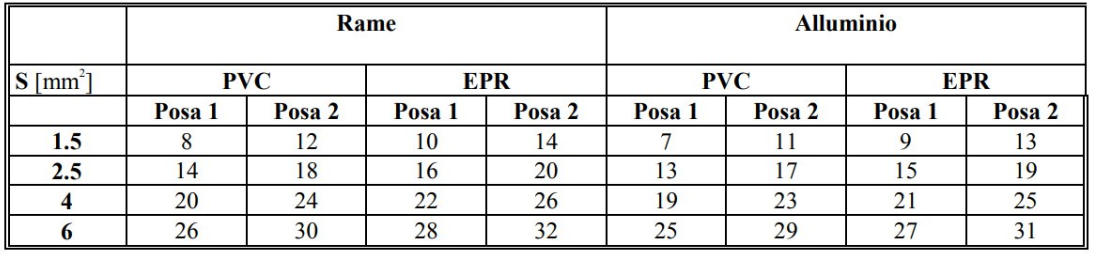
\includegraphics[width=0.8\linewidth]{immagini/dimensionamento_membrature15}
\end{figure}

Quando le condizioni operative differiscono dalle condizioni standard di prova, la corrente di impiego deve essere riscalata introducendo opportuni fattori correttivi moltiplicativi o divisori:
\begin{itemize}
    \item \textbf{Fattore di correzione per temperatura ambiente ($K_1$)}: se la temperatura effettiva di posa è pari a $X\,{}^\circ\text{C}$ (differente dai $30\,{}^\circ\text{C}$ nominali), la corrente di impiego viene normalizzata mediante la formula:
    \[ I_B(30\,{}^\circ\text{C}) = \frac{I_B(X\,{}^\circ\text{C})}{K_1} \]
    I valori di $K_1$ sono desunti da tabelle standardizzate in funzione dell'isolante (PVC o elastomerico/EPR), del tipo di posa (fissa in aria, fissa in terra, mobile) e della temperatura effettiva, spaziando da $10\,{}^\circ\text{C}$ a $65\,{}^\circ\text{C}$. La temperatura nominale di riferimento della specifica posa si individua in corrispondenza del valore $K_1 = 1{,}00$.
    \begin{figure}[H]
    	\centering
    	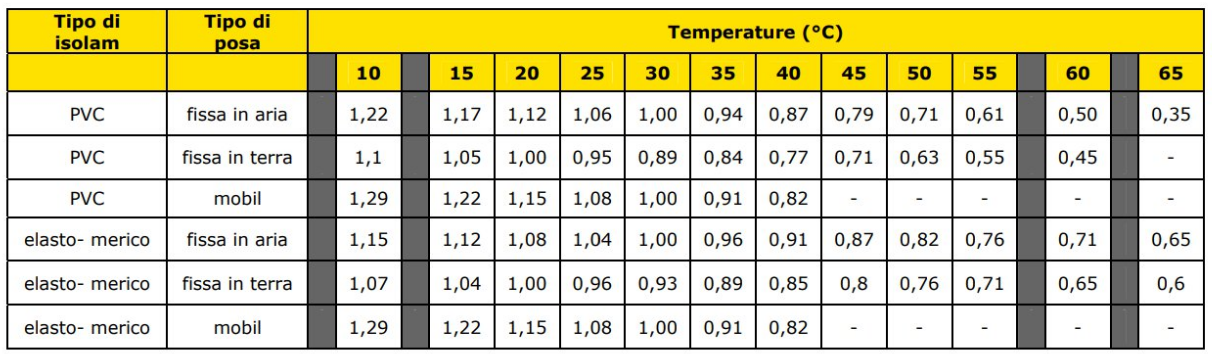
\includegraphics[width=0.8\linewidth]{immagini/dimensionamento_membrature16}
    \end{figure}
    
    \item \textbf{Fattore di correzione per modalità di posa ($K_2$)}: qualora la posa scelta $P_2$ non coincida con la configurazione di riferimento $P_1$ assunta nelle tabelle base, la corrente viene scalata mediante il coefficiente $K_2$ fornito dal costruttore:
    \[ I_B(P_1) = \frac{I_B(P_2)}{K_2} \]
    \item \textbf{Fattore di correzione per raggruppamento di circuiti}: la contiguità spaziale tra più cavi multipolari o conduttori unipolari posati su passerelle orizzontali riduce l'efficienza dello smaltimento termico per mutuo riscaldamento. Vengono applicati coefficienti riduttivi determinati in funzione del numero di passerelle verticali e del numero di terne o cavi affiancati orizzontalmente.
    \begin{figure}[H]
    	\centering
    	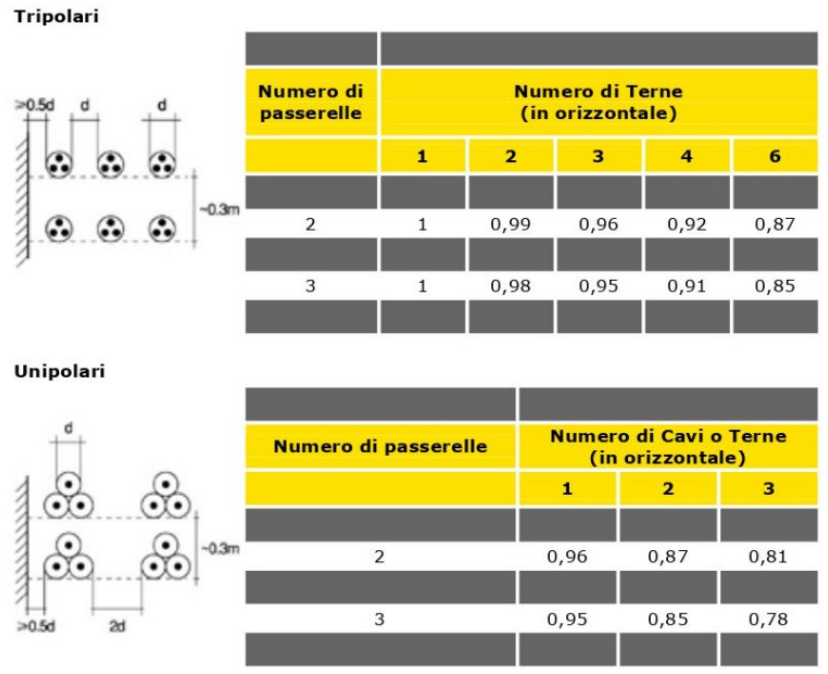
\includegraphics[width=0.6\linewidth]{immagini/dimensionamento_membrature17}
    \end{figure}
\end{itemize}